\documentclass{article}
\usepackage{fancyhdr}
\usepackage{lipsum}  
\usepackage{listings} 
\usepackage{xcolor}   
\usepackage{amsmath}
\usepackage{enumitem}
\usepackage{graphicx}
\usepackage{caption}
\usepackage{verbatim}

% Define macros for title and author
\newcommand{\thetitle}{STAT 641 \\ Homework 1}
\newcommand{\theauthor}{Keegan Smith}

\title{\thetitle}
\author{\theauthor}

\pagestyle{fancy}
\fancyhf{}  % Clear all header and footer fields
\fancyhead[L]{\nouppercase{\rightmark}}
\fancyhead[C]{\thetitle}  % Title in the center
\fancyhead[R]{\theauthor}  % Your name on the right

\lstset{ %
  backgroundcolor=\color{lightgray},   % choose the background color
  basicstyle=\ttfamily\small,          % size of fonts used for the code
  keywordstyle=\color{blue},           % color for keywords
  commentstyle=\color{green},          % color for comments
  stringstyle=\color{red},             % color for strings
  numbers=left,                        % where to put the line-numbers
  numberstyle=\tiny\color{gray},       % style for line-numbers
  stepnumber=1,                        % the step between two line-numbers
  numbersep=5pt,                       % how far the line-numbers are from the code
  frame=single,                        % adds a frame around the code
  rulecolor=\color{black},             % frame color
  breaklines=true,                     % automatic line breaking
  breakatwhitespace=false,             % automatic breaks should only happen at whitespace
  showspaces=false,                    % don't show spaces in the code
  showstringspaces=false,              % don't show spaces in strings
  showtabs=false,                      % don't show tabs in the code
}

\begin{document}

\maketitle

\section*{Question Group 1}
\begin{enumerate}
\item An observational study only collects information about subjects without giving treatments while an experimental study collects information about individuals who are given a treatment (and who are not given a treatment usually). \\
An example of an observational study is an election poll. \\
An example of an experimental study is a clinical trial. \\
\item Correlation in observational studies can often be misinterpreted as causation. This can be avoided by explicitly stating to your readers that there is no evidence of causation even if the data have strong correlation. \\
\item Probability sampling is when you assign a probability to each sample and select a random sample based on the assigned probabilities. Non-probability sampling is not random, samples are chosen by the researchers, not a random number generator. \\
An example of probability sampling is having a list of patients and flipping a coin for each patient. If heads, the patient is included, if tails the patient is not. \\
An example of non-probability sampling is selecting the next 50 people who walk in the store as samples. \\
\item Randomization in experimental studies to prevent unknown sources of biases. An example of when randomization is important is if the experiment could be affected by something like sunlight exposure. \\
\item Sampling error is the difference between the actual parameter of the population and the statistic collected from the sample. Non-sampling errors are errors that occur as a result of biases in the collection of the sample data. \\
An example of sampling error is when you collect a sample of incomes from US citizens and the average income you observed is less than the census data would suggest. \\
An example of non-sampling error is measurement bias: maybe you give out a survey and the questions are unclear. \\
\item a Prospective study makes an observation about a sample in the present and follows the subjects in the future to gather results. On the other hand, a retrospective study observes the sample in the present, and collections information about the subjects from the past. \\
An example of a prospective study is recording whether or not a subject was involved in the Head start program, and then following the subjects to see who achieves academic success. \\
An example of a retrospective study is collecting a sample of people who do and don't have colon cancer and then collecting information about their past diets. \\
\item Stratified sampling is when you divide the population into $L$ strata and select a random subset from each strata. Stratified sampling often results in smaller variance of sample means. An example of stratified sampling is dividing california into 20 regions and randomly selecting 10 oak trees to see the effect of feral pigs on vegetation. \\
\item confounding is when one or more effects cannot unambiguously be attributed to a single factor. An example of this can be found in scenario IV of the semi-conductor wafer experiment where they don't apply the thicknesses in a random fashion. Since they are changing the thicknesses one after another on the same wafer, effects could be attributed to the methodical changing of thicknesses as well as the thickness itself. \\
This would be fixed by randomly applying the thicknesses.\\
\end{enumerate}
\section*{Question Group 2}
\begin{enumerate}
\item Experimental, Comparative. The response variable is mathematics performance, the explanatory variable is teaching method. \\
\item Observational, Comparative. The response variable is the number of flu cases, the explanatory variable is the month of the year. \\
\item Experimental, Comparative. The response variable is plant growth, the explanatory variable is the light condition. \\
\item Observational, Descriptive.
\end{enumerate}
\section*{2.2}
\begin{enumerate}
\item Observational, Descriptive. \\
\item Experimental, Comparative. The response variables are crop yield and pest population and the explanatory variable is pesticide type. \\
\item Observational, Comparative. The response variable is income and the explanatory variable is level of education. \\
\item Experimental, Comparative. The response variable is memory recall, the explanatory variable is type of music.
\end{enumerate}
\section*{2.3}
\begin{enumerate}
\item Experimental, Comparative. The response variable is test score, the explanatory variable is time slept. \\
\item Experimental, Comparative. The response variable is brand preference, the explanatory variable is taste. \\
\item Experimental, Comparative. The response variable is air quality index, the explanatory variable is type of public transportation system \\
\item Observational, Comparative. The response variable is how they celebrate, the explanatory variable is the time of year. \\
\end{enumerate}
\section*{Question Group 3}
\begin{enumerate}
\item This is a stratified, multi-stage cluster sample \\
\item This is a multi-stage cluster sample \\
\item This is a systematic sampling \\
\item This is a stratified, multi-stage cluster sample \\
\end{enumerate}
\section*{3.2}
\begin{enumerate}
\item This is a stratified, multi-stage cluster sample \\
\item This is a systematic, multi-stage cluster sample \\
\item This is a stratified, systematic sample \\
\item This is a stratified, single-stage cluster sample \\
\end{enumerate}
\section*{Question Group 4}
\begin{enumerate}
\item Retrospective study, comparative. The response variable is the change in transportation usage, the explanatory variable is the new subway line. \\
\item Prospective study, comparative. The response variable is survival rate, the explanatory variable is treatment type. \\
\item Survey, descriptive. \\
\item Survey, descriptive. \\
\end{enumerate}
\section*{4.2}
\begin{enumerate}
\item Retrospective study, comparative. The response variable is sleep quality, the explanatory variable is diet. \\
\item Prospective study, descriptive. 
\item Retrospective study, descriptive. \\
\item Retrospective study, comparative. The response variable is test scores, the explanatory variable is curriculum. \\
\end{enumerate}
\section*{Question Group 5}
\begin{enumerate}
\item "fert A mean height: "
46.5 \\
"fert A mean tomatoes: " 
4.75 \\
"fert B mean height: "
41.5 \\
"fert B mean tomatoes: "
8.25 \\
"fert C mean height: "
51.625 \\
"fert C mean tomatoes: "
2 \\
\item Fertilizer C seems to be the best for increasing plant height. Fertilizer B seems to be the best for increasing the number of tomatoes. \\
\item Despite C having the best average height, it has the worst average number of tomatoes. Despite B having the best average number of tomatoes, it has the worst plant height. It seems that A is the sweet spot with its average height and number of tomatoes being second best of the fertilizers. \\
\item The weather is a confounding variable that could have affected the effectiveness of the fertilizers. Maybe some of the fertilizers do better or worse depending on the weather. This could be prevented by growing the plants indoors. \\
\item Graph: \\
\begin{figure}[ht]
  \centering
  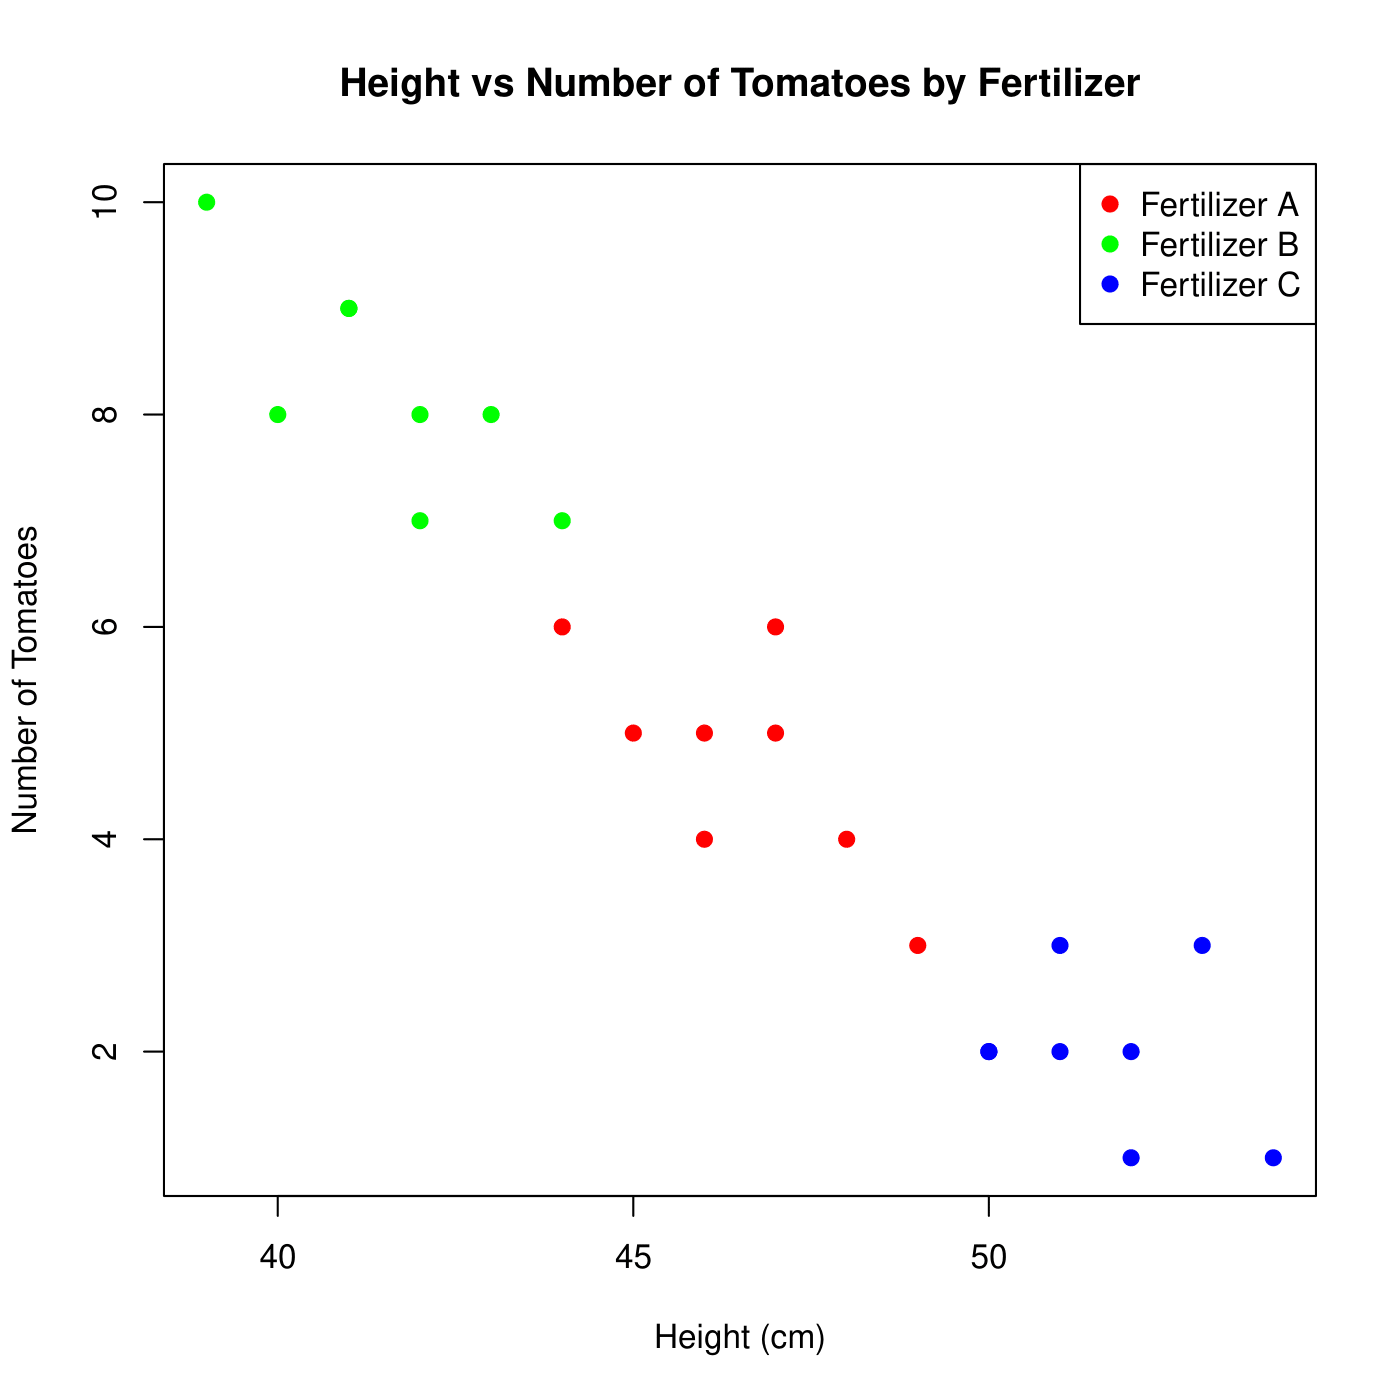
\includegraphics[width=0.7\textwidth]{Rplots-1.png}
  \label{fig:height_vs_tomatoes}
\end{figure}
\newpage
\item From the graph, you can see a vague inverse linear relationship between number of tomatoes and height. In general, as the height of the plant increases, the number of tomatoes decreases. We can also very clearly see that the fertilizers are very polarized with A, B, and C having few overlapping height and number of tomatoes values. \\
\item 
\begin{verbatim}
df <- read.csv("data.csv",
                header = TRUE, sep = ",")
head(df)

fert_A_df = df[df$Fertilizer == "A", ] 
print("fert A mean height: ")
mean(fert_A_df[["Height_cm"]])
print("fert A mean tomatoes: ")
mean(fert_A_df[["Number_of_Tomatoes"]])

fert_B_df = df[df$Fertilizer == "B", ] 
print("fert B mean height: ")
mean(fert_B_df[["Height_cm"]])
print("fert B mean tomatoes: ")
mean(fert_B_df[["Number_of_Tomatoes"]])

fert_C_df = df[df$Fertilizer == "C", ] 
print("fert C mean height: ")
mean(fert_C_df[["Height_cm"]])
print("fert C mean tomatoes: ")
mean(fert_C_df[["Number_of_Tomatoes"]])

#create the plot for height vs num tomatoes
plot(fert_A_df$Height_cm, fert_A_df$Number_of_Tomatoes,
     main = "Height vs Number of Tomatoes by Fertilizer",
     xlab = "Height (cm)", ylab = "Number of Tomatoes",
     pch = 19, col = "red", xlim = range(df$Height_cm),
     ylim = range(df$Number_of_Tomatoes))

#add fertilizers b and c to the plot with different colors
points(fert_B_df$Height_cm, fert_B_df$Number_of_Tomatoes, pch = 19, col = "green")
points(fert_C_df$Height_cm, fert_C_df$Number_of_Tomatoes, pch = 19, col = "blue")

#add a legend to the plot with the appropriate color fertilizer mapping
legend("topright",
       legend = c("Fertilizer A", "Fertilizer B", "Fertilizer C"),
       col = c("red", "green", "blue"),
       pch = 19)
\end{verbatim}

\end{enumerate}
\end{document}

